\section{Aim 3 --- Bluesky steering framework}
\label{sec:aim3}

\textit{Strawman owners: Campbell, with Allan, Maffettone, Caswell, Rakitin,
Barbour, Olds. $\sim$500 words.}

Aim~3 is the shared loop, not a new control system. The four steps in the
proposal are reduce, decide the next action, encode it to controls, and
collect. Two timescales sit inside that loop: faster than a measurement
(instrument optimization) and commensurate with a measurement (sequence
planning). Interoperation was specified with the Queue Server, workflow
systems, and parameterized similar measurements (for example powder). The UI
was specified to show the live experiment, agent state, history, queued plans,
and hyper-parameters \cite{allan2019bluesky}.

Bluesky was the reference implementation \emph{because} pieces can be adopted
without replacing a beamline. This paper should score that interop claim, not
assume a single stack won.

The 2023 ``Agents'' are pluggable modules in this pipeline --- local or
facility/HPC --- that consume reduced data and emit the next measurement or
control directive. Gaussian-process fly-scan demos at NSLS-II already existed
when the proposal was written. They are not language models.

\textit{Placeholders:} Bluesky/Tiled status; LCLS MFX photon-beam tuning and
operator-facing skills as one Aim~3 + Aim~1 crystallography cell.


\subsection{Bluesky-Adaptive: a short history}
\textit{Owner: Hopkins.}

Bluesky Adaptive, previously Blop (the Bluesky Optimization Package), began at NSLS-II
as a single-purpose tool: a custom-built wrapper around BoTorch for Gaussian-process 
Bayesian optimization. With little integration into Bluesky itself, it was purely
for autonomously aligning a beamline by maximizing a measured figure of merit. That 
design was published in the Journal of Synchrotron Radiation in 2024 as a general 
algorithm for autonomous beamline alignment \cite{Morris2024}. Starting in 2025, 
the project outgrew that single-purpose shape and became a general-purpose steering 
toolbox for Bluesky.

That work did two things at once: it replaced the hand-built BoTorch wrapper with
Ax, which handles trial generation and experiment tracking on top of BoTorch; and
it separated the optimization logic from the Bluesky-facing code behind a small
set of protocols, so that a plan-facing half that only knows how to run a Bluesky
acquisition and evaluate its outcome stays separate from an optimizer-facing half
that proposes the next point, checkpoints its state, and recovers from a failed
trial. Once that boundary existed, Blop became a bridge between optimizer backends
and Bluesky, via those protocols and the plans built on them, rather than a single
Ax/BoTorch agent: new backends could be added without touching the Bluesky side,
including a classical SciPy backend (local minimization, SHGO, dual annealing) for
problems that do not need a surrogate model, and an Xopt backend, alongside the
Ax/BoTorch Bayesian optimizer.
% protocols diagram with short description about minimal borders between modules
The same year of work hardened Blop for the kind of unattended, remote operation a
multi-facility steering framework needs: optimizer state can be checkpointed and
restored, a failed evaluation no longer stalls a run, and an optimization can stop
itself against a global criterion instead of a fixed trial count. Its integration
with the Bluesky Queue Server grew from an experimental add-on into a restartable,
checkpointable component that can run on a remote queue unattended. None of this
removed the experimenter from the loop: an operator can still override a suggested
point manually, and review model fit and uncertainty before a move is committed.

\begin{figure}[t]
\centering
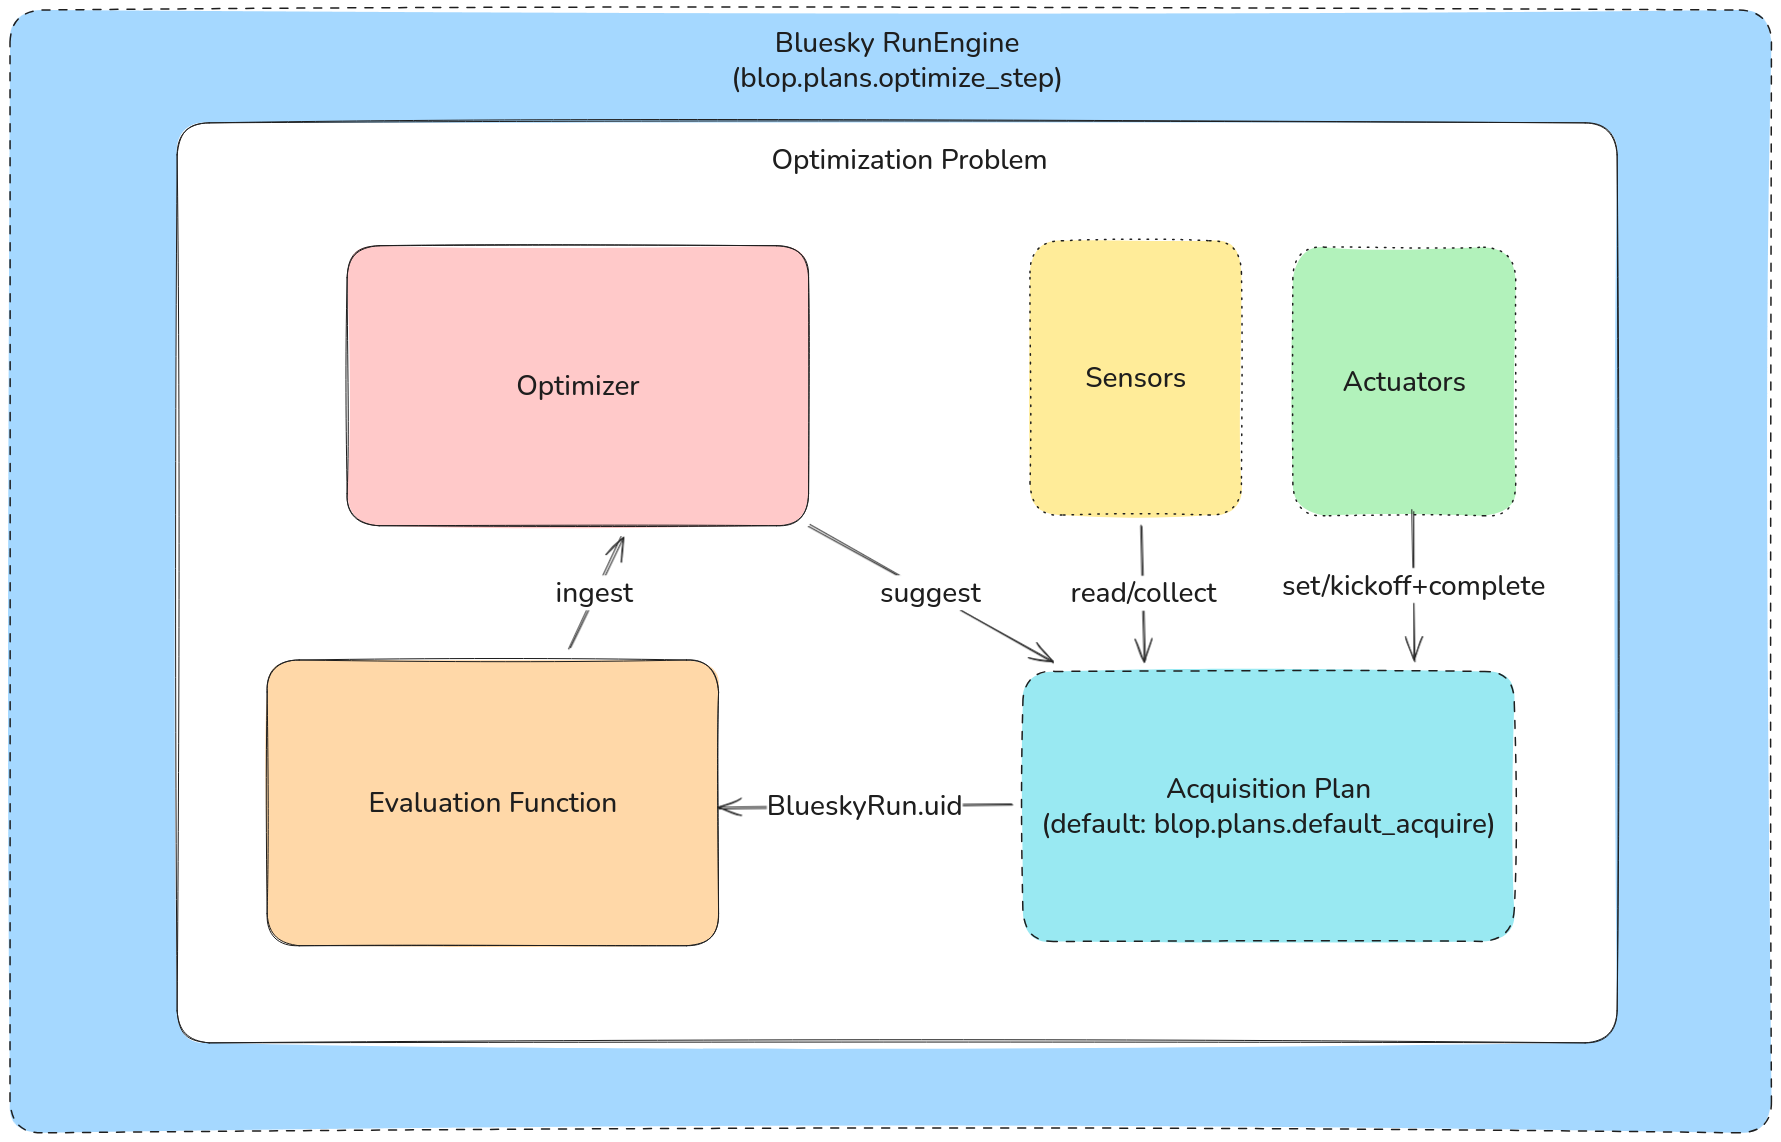
\includegraphics[width=\linewidth]{src/figures/blop_protocols.png}
\caption{Bluesky-Adaptive separates optimizer logic from the Bluesky acquisition path: the optimizer proposes the next action, while a plan reads sensors, collects data, and issues actuator commands through the standard RunEngine flow.}
\label{fig:blop_protocols}
\end{figure}

Blop also grew as a project rather than just as code: it moved out of a single
facility's repository into the shared \texttt{bluesky} GitHub organization,
reached its first stable 1.0 release in mid-2026, and is now packaged for both PyPI
and conda-forge. What began as one beamline's alignment script is now a shared,
multi-backend building block for the decision-support layer this Aim describes.

The next step builds on that same core rather than replacing it: Blop's
protocol-based architecture is migrating into \texttt{bluesky-adaptive}, enabling
service-oriented deployment and passive, off-policy learning agents alongside the
online optimizers described above. Once that migration lands, the Blop package
itself will be archived; the architecture built over the past year carries forward
unchanged.

\subsubsection{Bluesky-Adaptive v1.0 Release}

The July 2026 version 1.0 release has improved Bluesky-Adaptive's usability and accessibility 
for both users and developers. Through improved documentation, which includes detailed 
hands-on tutorials, active deployment references, and comprehensive how-to guides, Bluesky-Adaptive 
has become easier to adapt into new and existing workflows.
Functionality has also improved through the inclusion of scalarized multi-objective optimization 
support, manual data point injection and data priming, best-point navigation, and configurable 
stopping criteria, providing operators finer control over trial execution.
New first class support for Xopt and Scipy extend simple implementation utilities outside the 
Ax ecosystem, and incorporates several new domains of optimizers to the package.
Finally, simulation capabilities were expanded with a bring your own beamline workflow ideology 
using XRT, allowing for testing before actual beamtime is used.

\subsubsection{Bluesky-Adaptive-sim and XRT}

Bluesky-Adaptive-sim is a currently in development add-on to Bluesky-Adaptive targeting offline tuning and deployment
testing. Deployment of Bluesky-Adaptive workflows require discretionary beamtime like classical 
experiments to validate their performance, and the less time needed to do online setup the 
more algorithmic tuning and optimizer configuration can be done. There are also deployment
factors which can easily be covered with a rough simulation of the beamline ie:  

\begin{itemize} 

\item Do evaluation functions work and provide the correct cost?  

\item Are we in an order of magnitude of the correct bounds (is an axis too sensitive)?  

\end{itemize} 

This drives us to develop a "Beamline in a Box" system as an aggressively scaled semipermanent 
simulation, which acts as an "as best" software indistinguishable setup allowing for accurate, 
rapid, and reconfigurable offline deployment testing. We target swapout at the epics channel 
layer as it is a convenient flat low-level interface to mock a beamline through, with opaque 
self contained scalars providing an interface for arbitrary simulation complexity.

\begin{figure}[!htbp]
\centering
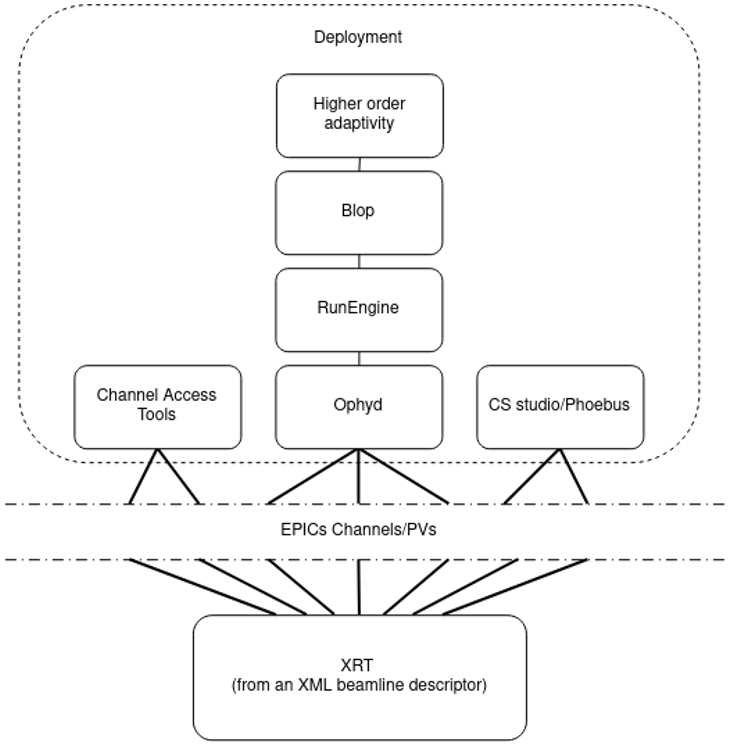
\includegraphics[width=0.82\linewidth]{src/figures/beamline_in_a_box.png}
\caption{Beamline-in-a-Box emulates a beamline behind the standard EPICS control interface, enabling Bluesky workflows to be tested offline before costly beamtime is used.}
\label{fig:beamline_in_a_box}
\end{figure}

\subsubsection{Beamline digital twins}
Two important use-cases motivate developing digital twins of synchrotron beamlines. 
First, a calibrated digital twin would allow the offline testing described above, optimizers 
such as Bluesky-Adaptive could be tuned, and candidate motor settings evaluated, \emph{in silico} 
without (or with limited) beamtime, to find optimal controls that are transferrable to the real 
beamline. 
Second, twins are also useful for understanding how a beamline behaves during operations. 
To accomplish this, a digital twin must be  {\it calibrated}: it must have  the right physics and 
parameters, and take the same motor positions as input as the real beamline. We have developed a 
differentiable calibration framework for building such a twin from motor and beam images pairs, 
and we have tested it on a routine grid scan of a real beamline at NSLS-II. The twin combines the
XRT ray-tracing simulator,  a learned map from motor positions to the poses of the optical elements, 
and a model of the camera. The framework is built on differentiable models such as neural networks 
(including a surrogate of XRT) which enable end-to-end differentiable learning (calibration) of the 
motor and detector models, and simulator parameters. On a $13^4$ scan of the KB mirrors at the TES 
beamline (NSLS-II), with only 32 frames the twin predicts held-out beam shapes as accurately as a 
data-only network trained on 512.
Future work will include studying the different sources mismatch between the digital twin and the real beamline.



\subsubsection{Bluesky-Adaptive deployments}
Bluesky-Adaptive has been deployed across multiple NSLS-II beamlines for a diverse set of optimization tasks.
These deployments were generally successful, but they also exposed the practical challenges that
frequently accompany machine-learning-driven control, including hyperparameter selection,
appropriate variable bounds, and robust evaluation metrics. They also highlighted issues that are
more specific to large user facilities, where beamtime is scarce and the cost of a failed or poorly
tuned online optimization is high.

At CHX, Bluesky-Adaptive has been used to optimize Bragg-peak finding with an imperfect Diamond, using the
FWHM and peak intensity of rocking curves to identify an optimal surface position. In that
setting, Bluesky-Adaptive improved acquisition efficiency by approximately 90\% relative to a brute-force
grid-scan strategy. At XPD, ongoing work demonstrates the broader potential of the framework for
autonomous experimental workflows, including integration with the Bluesky Queue Server. Taken
together, these examples show that the method is not limited to a single optimization problem but
can adapt to different beamline workflows and measurement constraints.

An earlier deployment at BMM was less successful and illustrates the gap between an optimization
concept and a robust beamline operation. Such experiences reinforce the importance of realistic
simulations, carefully defined objective functions, and physically meaningful parameter bounds
before committing valuable beamtime.

Taken together, these deployments demonstrate both the capabilities of Bluesky-Adaptive and the practical
considerations required to deploy optimization reliably in real experimental environments. 